\chapter{Theorethical Foundations}\label{chapter:theorethical}
\section{Multicore Systems}\label{section:multicore}
Until the beginning of the 2000's the advances in processors technology were made through improvements in the single CPU performance. These advances allowed the increase in the clock speed of a the processors. Given the fact that the heat generated by a transistor is proportional to its operating frequency,the high clock frequencies reached led to a great amount of dissipated heat that could not be easily handled. In order to decrease the consumed power and take advantage of the increasing transistor count in every chip, the industry decided to incorporate multiple CPUs with a moderate performance instead of a single one with a high frequency and therefore power consumption. This new design trend is known as multicore. 

In a single CPU the executing code can be executed in a more efficient way by the CPU by using mechanisms such as the reordering of instructions. With the appearance of multicores there is a greater demand on the programmer to write code that can exploit all the available capacity offered by the processor. Part of this increasing programming effort consists of allowing the code to execute in units called threads, where a n core CPU has the capacity to execute n threads simultaneously. This expression of code in threads can be explicitly done with the help of frameworks such as pthreads or can be done implicitly by annotating regions of code that can be parallelized using tools such as OpenMP.

\subsection{Thread pinning}\label{subsection:pinning}
Given a code that executes in n threads using a processor with m cores, we would like to have the ability to control which executing core will be used to execute a given thread. The mapping of an executing thread to a hardware core is known as thread pinning or thread affinity.

There are many mechanisms available to set the pinning of a program, such as:

\begin{itemize}
	\item In OpenMP the environment variable GOMP\_CPU\_AFFINITY=a,b,c,… sets the affinity of a program as a list where a,b and c represent the identifiers of the cores that will execute the thread with the id in the position in which the identifier was given. In this example thread 0 will be executed in core a, thread 1 in core b and so on.
	\item In numactl the parameter physcpubind can specify in a similar manner as is done in OpenMP, as a listing of the desired cores.
	\item In Autopin+ the user specifies many possible pinnings, and the tools will explore these combinations of pinnings for the most optimal in terms of execution speed.
\end{itemize}
Pinning can play a very important role in the performance of a program. In many cases distributing a thread to a free core might yield the best performance, but in other scenarios -especially in NUMA systems- this might not be the case depending of the locations of memory accesses by the thread, these factors will be explored later in more depth. 

\section{The bus interface and multicore systems}\label{section:businterface}
\begin{figure}
	\centering
		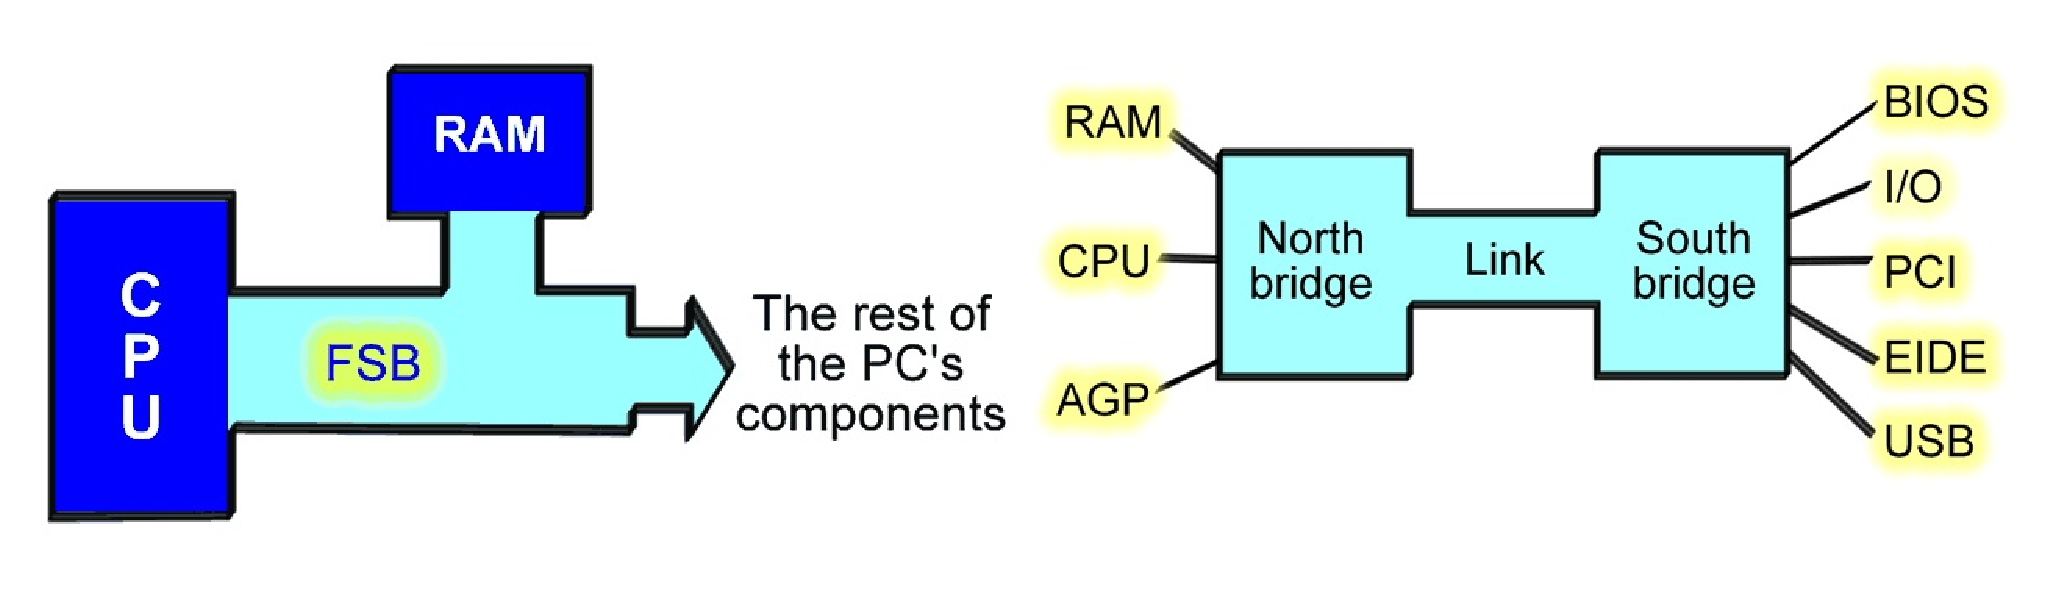
\includegraphics[width=.9\textwidth]{figures/bus-abstraction.eps}
		\caption[bus-abtraction]{Abstraction of the data traffic between the CPU and the external entities. The left hand side abstracts the RAM as being closer to the cpu than the other components, and the other shows a more accurate description with the Northbridge and Southbridge chips redirecting the traffic. Image Karbosguide \cite{pcarch-carbo}. }
		\label{fig:bus-abs}
\end{figure}

In earlier computer systems, the processor chip had a communication with the memory through a high speed path called the Front Side Bus(FSB), which connects the last level of cache of a processor chip with the memory controller. This front side bus also allows the communication between the processor chip and other peripherals through the Northbridge chip. This layout means that all the traffic between the processor and the exterior world was centralized through the front side bus, but in many cases a great share of the traffic is occupied by the memory-processor data. The visualization of this layout is given in figure \cite{fig:pcarch-carbo}. 

Given the always present need to optimize the supply of memory data to the CPU, this front side bus scheme has been changed and a quicker way for the CPU to access memory has been devised, these improvements can be seen in the form of higher bandwidth and low latency . Nowadays the path between the processor and the memory controller has been taken in-chip, which means that the processor has a straight path to the memory controller inside the same silicon die. In many modern multicore processors, specifically those from Intel and AMD, every core has its own L1 and L2 caches and all the cores share the L3 or last level cache. With the introduction of the dedicated memory access interface every processor chip has a part not specific to any core which handles the access to memory, in Intel technology this in-chip intermediation area is known as the uncore.

\section{Multiprocessor Systems}\label{section:multiproc}

\begin{figure}
	\centering
		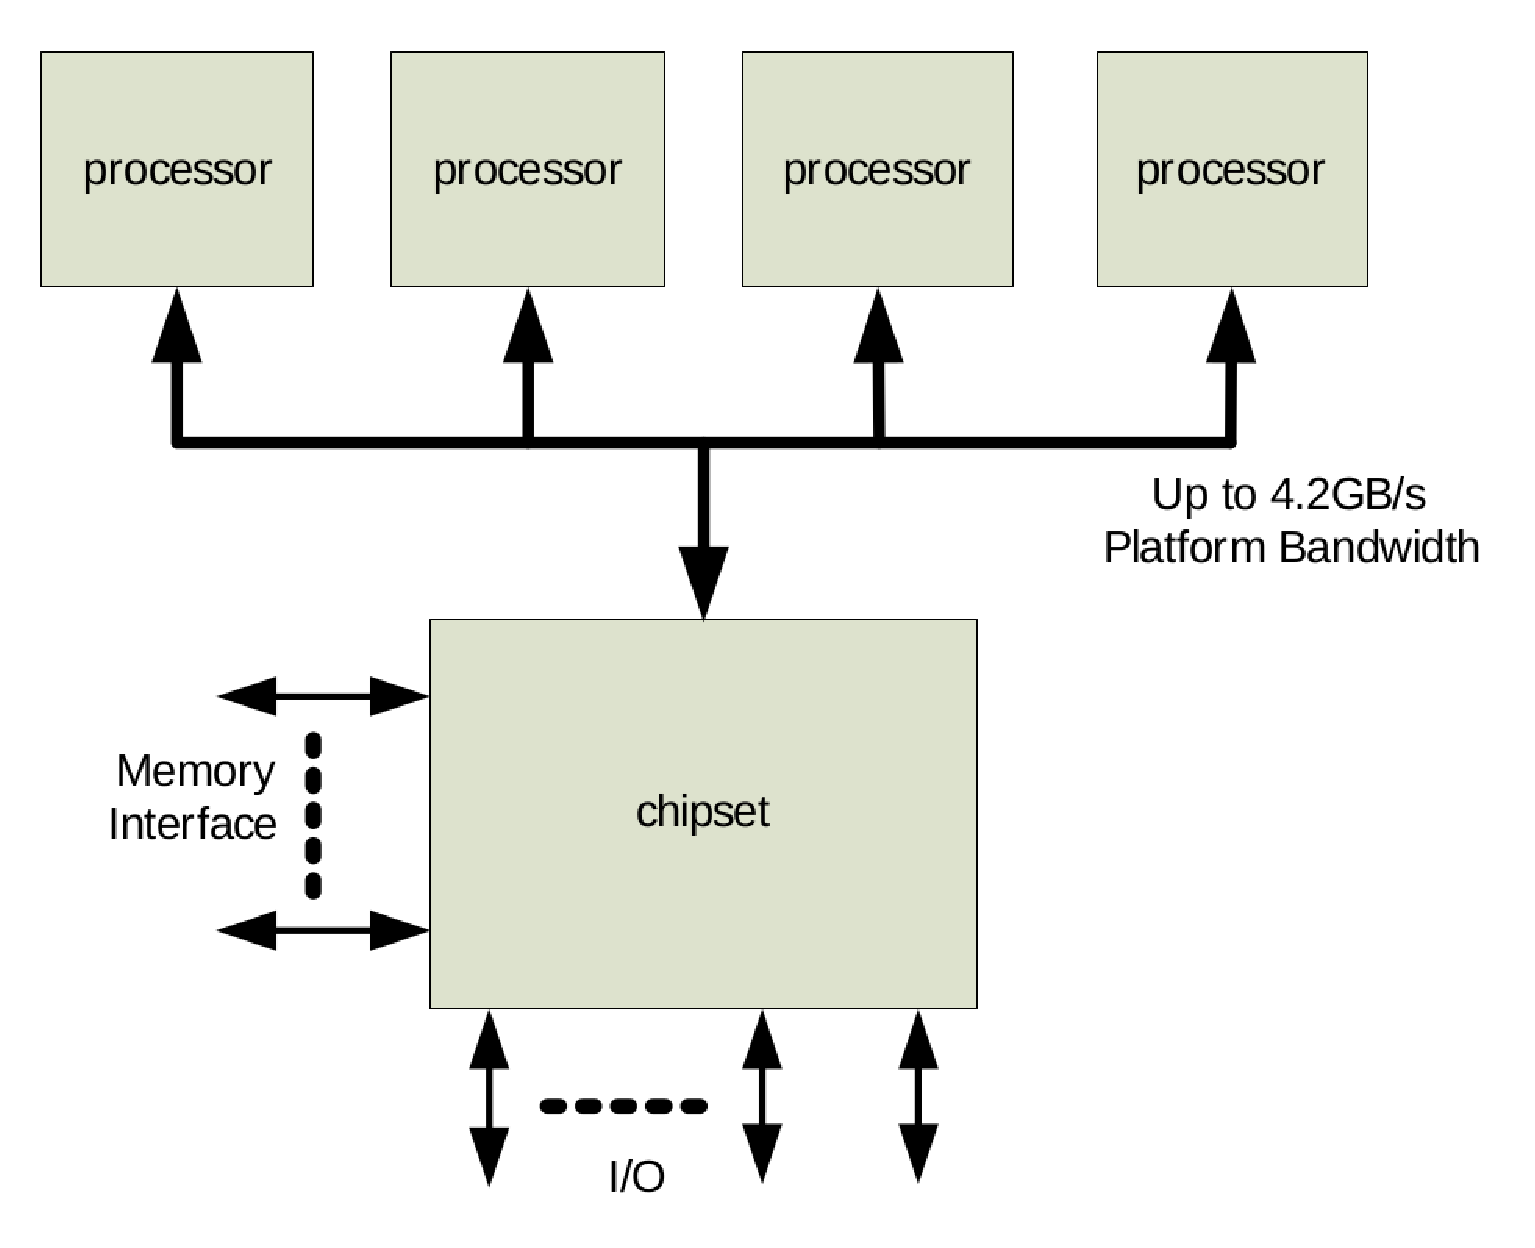
\includegraphics[width=.6\textwidth]{figures/uma1.eps}
		\caption[basic-uma]{Basic UMA System with the Frontside Bus as an unifying element. Image Intel Corporation \cite{qpi-intel}. }
		\label{fig:uma1}
\end{figure}

In situations where the power of a single processor computer is not enough -even if this processor is a multicore- it might be possible to incorporate in a computer system multiple processor chips. Usually in such multichip systems all the memory can be accessed by any of the participating processors. As the cores see a global memory space, it is possible that two processes access the same memory location at the same time. In this simultaneous access case it is advisable that when one processor writes over a memory location the other processors -even the ones located in other chip- see this change as well. This concept of keeping a synchronized version of a shared memory location is known as cache coherency. 

In earlier multiprocessor systems the sharing of data between processors was done through a connection to the Front Side Bus, where memory can be accessed through the chipset (Northbridge) as shown in the Figure \cite{fig:uma1}. This shared bus topology meant that all memory accesses are treated equally no matter which processor accesses it, thus guaranteeing properties such as the latency of an access. This equality of accesses leads that this type of interconnection is known as an Uniform Memory Access. Later some enhancements were made to this architecture such as the segmentation of the shared buses and joining of these separate buses through cache coherency enforcement hardware.

\subsection{Numa systems}\label{subsection:numa}

\begin{figure}
	\centering
		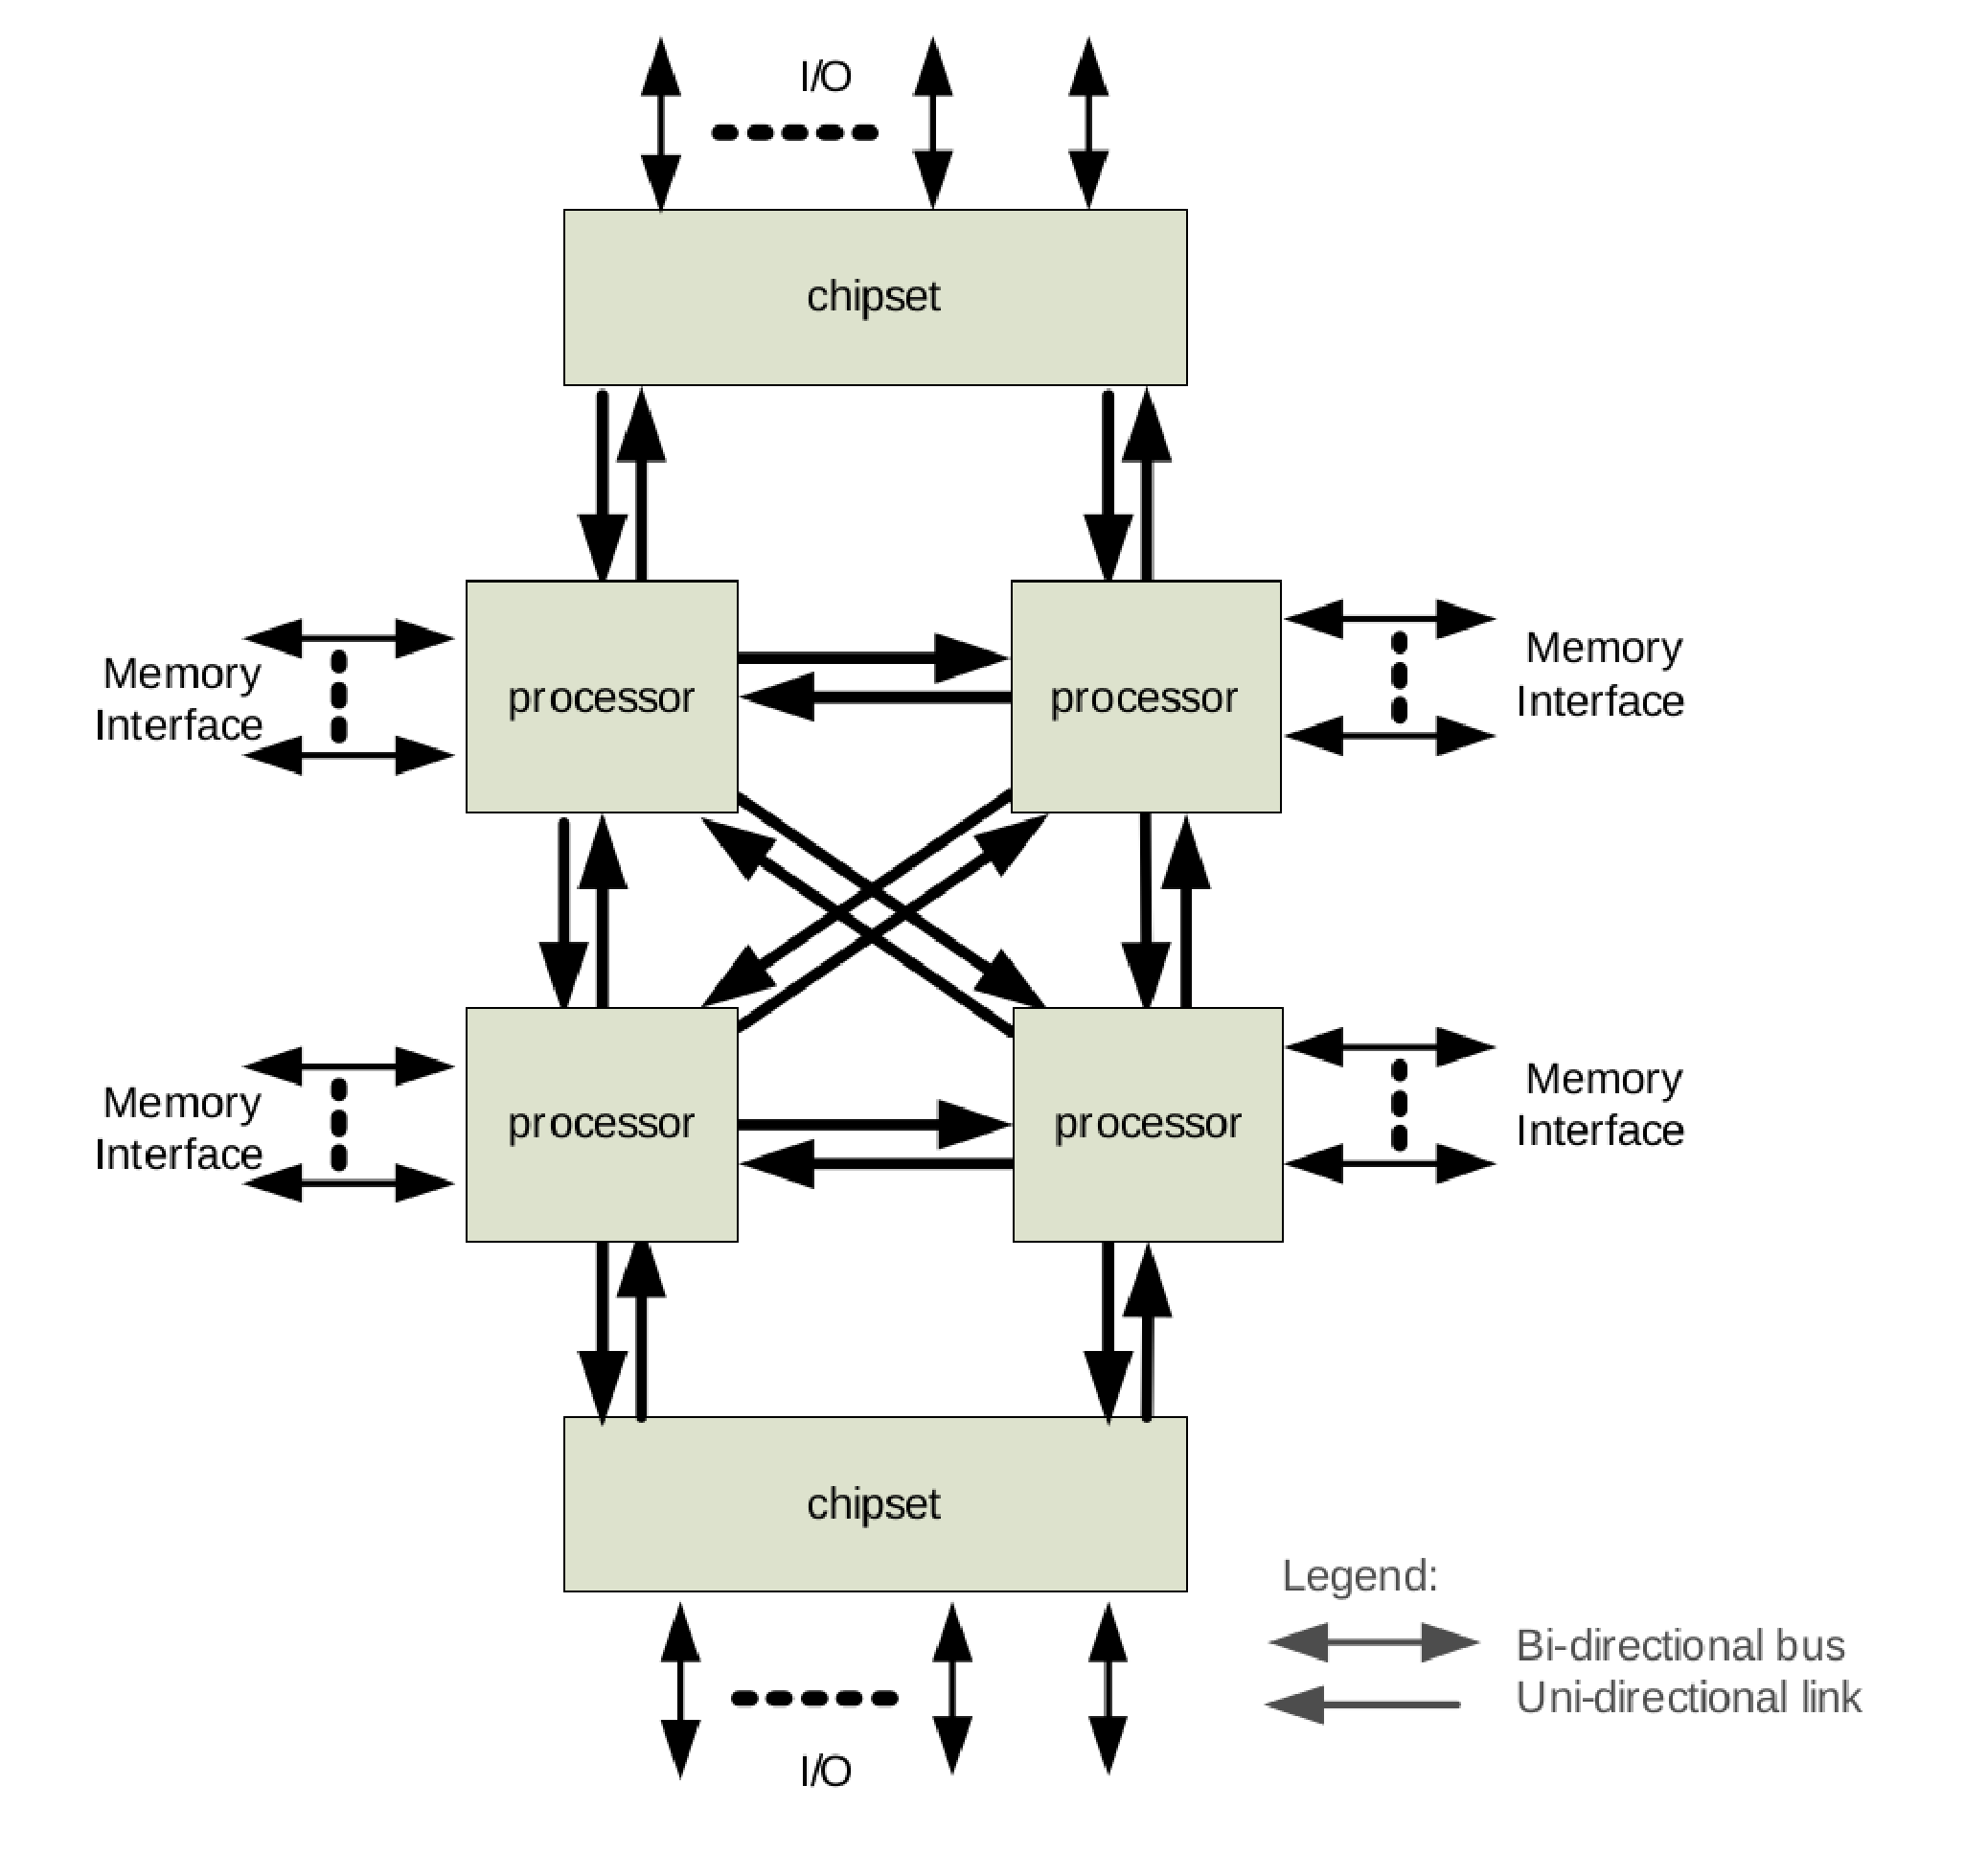
\includegraphics[width=.6\textwidth]{figures/numa-qpi.eps}
		\caption[basic-uma]{Numa system with four nodes with a QPI interconnection. Image Intel Corporation \cite{qpi-intel}. }
		\label{fig:numa1}
\end{figure}

Although the interconnection through the Front Side Bus provides very firm guarantees about the access time it has a very obvious downside, which is the bottleneck that could be produced when all the memory accesses are conducted through a single path. This bottleneck, together with the need to give the processor more memory access bandwidth with less latency has led to the development of point to point connection between processors. Instead of being just a bus protocol these processor-memory links have taken the form of a layered protocol with packetized units of communication specific to every manufacturer. The most common forms of this new interface are Intel's Quick Path Interconnect and AMD's HyperTransport technologies. Figure \cite{fig:numa1} shows the representation of an Intel NUMA system interconected using QPI.

With the introduction of the point to point interconnects a processor faces two options when given the task of making a memory access: either the desired location resides in its attached memory or it must fetch the location from a remote processor. A remote memory access has more latency than a local one due to the interprocessor transport involved in the transaction, which leads to remove the guaranteed access latency given in the UMA system. This latency guarantee cannot be held anymore because of the placement of the threads and memory pages in a multiprocessor system can be easily changed thus introducing the NUMA architecture, which stands for: Non uniform memory access. 

\section{Computer performance measurement}\label{section:perfmeas}

Modern computers are complex systems and there are multiple factors that might contribute to a degradation in system performance. The addition of performance counters, as they are usually called, allows to help track occurrences that happen inside a processor. These occurences can be for example cache or TLB misses, memory loads, instructions retired from the pipeline, among others.By reading these values it becomes possible to analyze where a bottleneck could be taking place. The performance tracking facilities are commonly referred to as the Processor Management Unit.

In modern CPUs the number of available counters is fixed, where every counter is programed by assigning it an event such as the ones mentioned above. The set of available events for every processor varies depending on the microarchitecture and it is usually found on the programming manual. 

\subsection{Instruction sampling}\label{subsection:sampling}
In the performance analysis of an algorithm sometimes it is desirable to associate the occurrence of an event with the instruction that caused it. Due to the great number of instructions executed by a processor it is not possible to keep track of every one of them, the strategy to apply here is to register information every certain number of instructions and extrapolate the results to the execution of the whole program. This follows the techniques of Statistical sampling and thus it is called the instruction sampling.

The first sampling versions of instruction sampling that appeared in Intel and AMD processors sometimes had trouble with associating the exact event measured with the instruction in a precise manner which caused a deviation in the association between the instruction and the event. Later, a revised version of the technology eliminated this shortcoming and it is present in AMD and Intel processor with the proprietary names of Instruction Based Sampling and Precise Execution Based Sampling. 